\documentclass[tikz]{standalone} 
\usetikzlibrary{hobby} 
\begin{document} 
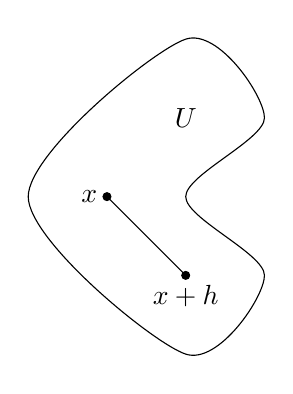
\begin{tikzpicture}[use Hobby shortcut]
\begin{scope}
%\clip (-5,-3.1) rectangle (5,3.1);
%\draw (0,0) .. +(1,0) .. +(1,2) .. +(1,3) .. +(0,3) .. (0,0); 
%\draw (-3,0) .. (-2,-2) .. (0,-1) .. (3,1) .. (0, 3) .. (-3,0); 
%\tikz [ closed  hobby ]  \draw  plot  coordinates  {(-3 ,0)  (0 ,-3) (3 ,0)  (0 ,3)};
\draw plot [smooth cycle] coordinates {(-2,0) (0,-2) (1,-1) (0,0) (1,1) (0,2)};
\node at (0,1) {$U$};
\draw[fill] (-1,0) circle [radius=0.05];
\node[left] at (-1,0) {$x$};
\draw[fill] (0,-1) circle [radius=0.05];
\node[below] at (0,-1) {$x+h$};
\draw (-1,0) -> (0,-1);
\end{scope}
\end{tikzpicture} 
\end{document}    